\documentclass[12pt]{article}
\usepackage[a4paper,
            bindingoffset=0.2in,
            left=1in,
            right=1in,
            top=1in,
            bottom=1in,
            footskip=.25in]{geometry}
\usepackage{amsmath}
\usepackage{amsfonts}
\usepackage{tcolorbox}
\usepackage{cancel}
\usepackage{bbm}
\usepackage{hyperref}
\hypersetup{
    colorlinks=true,
    linkcolor=blue
    }
\usepackage{enumitem}
\usepackage{physics}
\usepackage{amssymb}
\usepackage{pgfplots}
\pgfplotsset{width=10cm,compat=1.9}
\usepgfplotslibrary{fillbetween}
\usetikzlibrary{patterns}
\usepackage{amsthm}
\usepackage{graphicx}
\newcommand*{\T}{\mathrm{T}}
\newcommand*{\D}{\mathrm{D}}

\theoremstyle{definition}
\newtheorem{definition}{Definition}[section]
\newtheorem{example}{Example}[section]
\newtheorem{theorem}{Theorem}[section]

\title{{Introducing the tangent space} \\ \large{Mathematics of Machine Learning}}
\author{Evgenii Samutichev}

\begin{document}
\maketitle

\setcounter{section}{3}
\setcounter{definition}{13}
\setcounter{theorem}{14}

\begin{definition}\hypertarget{D1}
    Let $\mathcal{M}$ be a \textbf{subset} of $\mathcal{E}$. For all $x \in \mathcal{M}$, define 
    $$
    \T_x \mathcal{M} = \{c^\prime (0) \ | \ c : I \to \mathcal{M} \text{ is smooth and } c(0) = x\}
    $$
    where $I$ is any open interval containing $t = 0$. That is, $v \in \T_x \mathcal{M}$ if and only if there exists a smooth curve on $\mathcal{M}$ passing through $x$ with velocity $v$.
\end{definition}

\noindent \textbf{Discussion} The introduced set of vectors $\T_x \mathcal{M}$ will later be called the \textbf{tangent space} to $\mathcal{M}$ at $x$. And if we draw this for a sphere, we see that it makes a lot of sense. In particular, latitude and longtitude lines may be viewed as curves providing basis vectors for this space 
\begin{figure}[h!]
    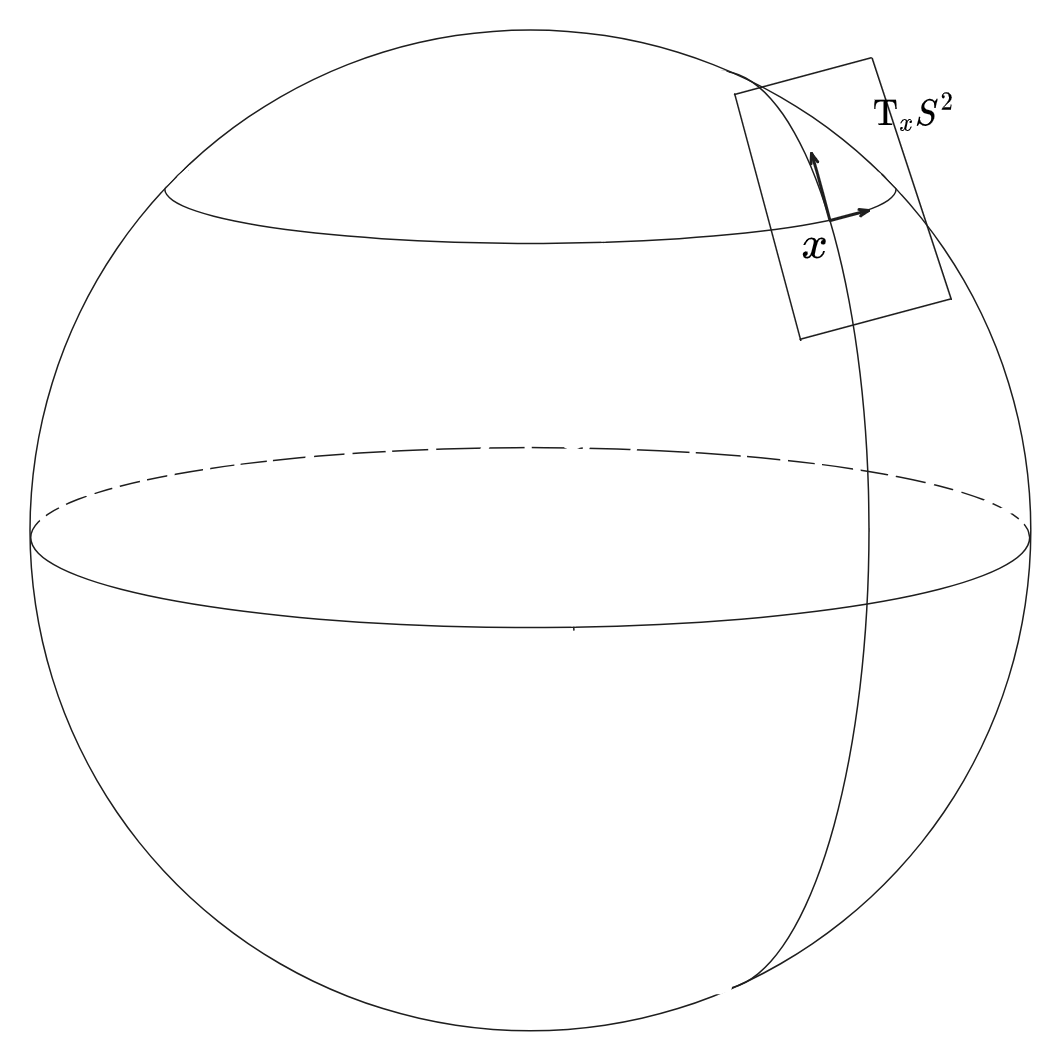
\includegraphics[width=0.3\textwidth]{figures/2.png}
    \centering
\end{figure}

Notice how it's defined for a set $\mathcal{M}$, which might not be a manifold. This is similar to how in real analysis we are comfortable with having piecewise-smooth curves s.t. they don't have tangent line everywhere. Ok, but you might reasonably ask: 

\textit{Haven't we defined the tangent space before through the kernel of the differential?} 

The answer is: we sort of defined it, but this definition is much better since it is \textbf{coordinate-free} (and there is this whole program in differential geometry to replace coordinate dependent definitions). What that means, is that if you want to define the tangent space through the kernel of the differential for $n=d-k$-dimensional manifold, you'll need this local defining function $h : U \to \mathbb{R}^k$ at $x$. And what if it so happens, that when you take some other local defining function $\tilde{h}$, then the resulting tangent space will be different? This is not obvious at all, and I'll give you an example in a minute, but we still have some more things to discuss here. 

So, the second question you might want to ask: 

\textit{Is it really a vector space?} 

The thing is, we can't really "add" curves. If there are two smooth curves providing us vectors $v_1$ and $v_2$, can we always construct a smooth curve passing through $x$ with velocity $v_1 + v_2$? When $\mathcal{M}$ is not a manifold, this problem will arise. Consider the following set $\mathcal{M}$ 
\begin{figure}[h!]
    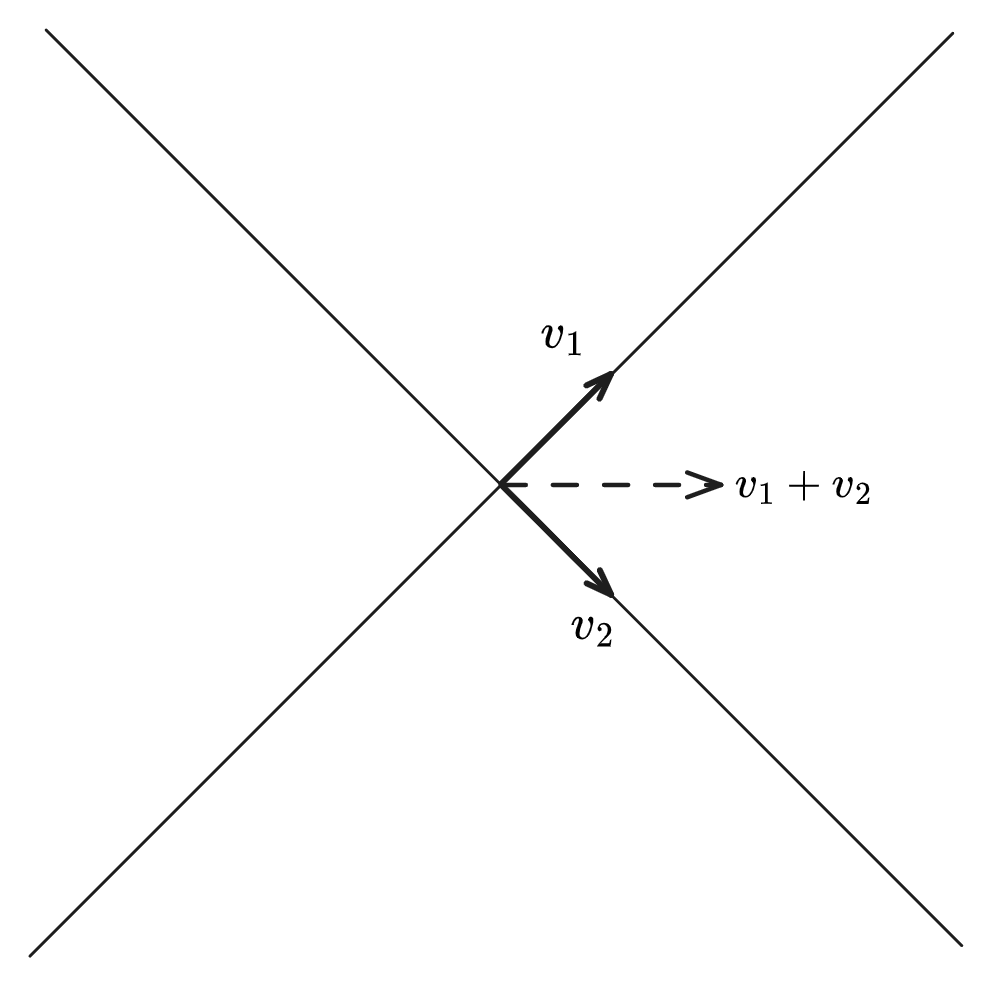
\includegraphics[width=0.29\textwidth]{figures/1.png}
    \centering 
\end{figure}

Notice that there is a singularity at the origin, and so for two vectors that are clearly in $\T_x \mathcal{M}$ their sum is not. 

Now, I want to show you by providing an example that the uniqueness of the tangent space is not obvious. 
$ $ 

\noindent \textbf{Example} Let's consider 
\begin{equation}
    S^{1}= \{(x, y) \in \mathbb{R}^2 \ | \ x^2 + y^2 = 1 \}
\end{equation}
and notice that for $x \neq 0$
\begin{equation*}
    x^2 + y^2 - 1 = 0 \Leftrightarrow x^3 + x y^2 - x = 0
\end{equation*}
then 
\begin{align}
\begin{split}
    h(x, y) &= x^2 + y^2 - 1 \\
    \tilde{h}(x, y) &= x^3 + x y^2 - x 
\end{split}
\end{align}
both are local defining for $S^{1}$ everywhere except $(0, \pm 1)$.

We can compute that 
\begin{equation}
    \D h(x, y)[v] = 2x v_x + 2y v_y
\end{equation}
and 
\begin{equation}
    \D\tilde{h}(x, y)[v ] = (3x^2 + y^2 - 1) v_x + 2xy v_y 
\end{equation}

\textit{Q: Just by looking at this, are you immediately convinced that the kernels of these two linear transformations are the same?}

For points satisfying $x^2 + y^2 = 1$ the second linear map can be written as 
\begin{equation}
    \D\tilde{h}(x,y)[v ] = 2x^2 v_x + 2x y v_y 
\end{equation}
so 
\begin{equation}
    \D\tilde{h}(x, y) = x \D h(x, y) 
\end{equation}

Although clearly 
\begin{equation}
    \D h(x, y) \neq \D\tilde{h}(x, y)
\end{equation}
but 
\begin{equation}
    \ker \D h(x, y) = \ker \D \tilde{h}(x, y)
\end{equation}
which wasn't initially obvious, since we had to perform certain transformations to achieve this. For $(x, y) \notin S^1$ this isn't even true in general. 

Now look back at the \hyperlink{D1}{Definition 3.14}. We clearly don't use any local defining function $h$ in it, it only involves the concept of a smooth path on the manifold, which is intrinsic to its geometry, and not to a particular choice of its coordinate representation. And keep in mind that we call it \textit{the} tangent space, which implies that it's unique. But, again, are we sure about that?

The following theorem provides the connection between our intuitive definition and the actual definition of the tangent space, while answering questions asked in the beginning of the lecture. 
\begin{theorem}
    Let $\mathcal{M}$ be an embedded submanifold of $\mathcal{E}$. Consider $x \in \mathcal{M}$ and the set $\T_x \mathcal{M}$. Then 
    \begin{enumerate}
        \item If $\mathcal{M}$ is an open submanifold, then $\T_x \mathcal{M} = \mathcal{E}$ 
        \item Otherwise, $\T_x \mathcal{M} = \ker \D h(x)$ with $h$ \textbf{any} local defining function at $x$
    \end{enumerate}
\end{theorem}

\noindent \textbf{Discussion} But before we get to the proof, I would like to briefly remind you the geometric side of \textbf{Theorem 3.12} from the previous lecture. 

As an example, let's look at a sphere again. 
\begin{figure}[h!]
    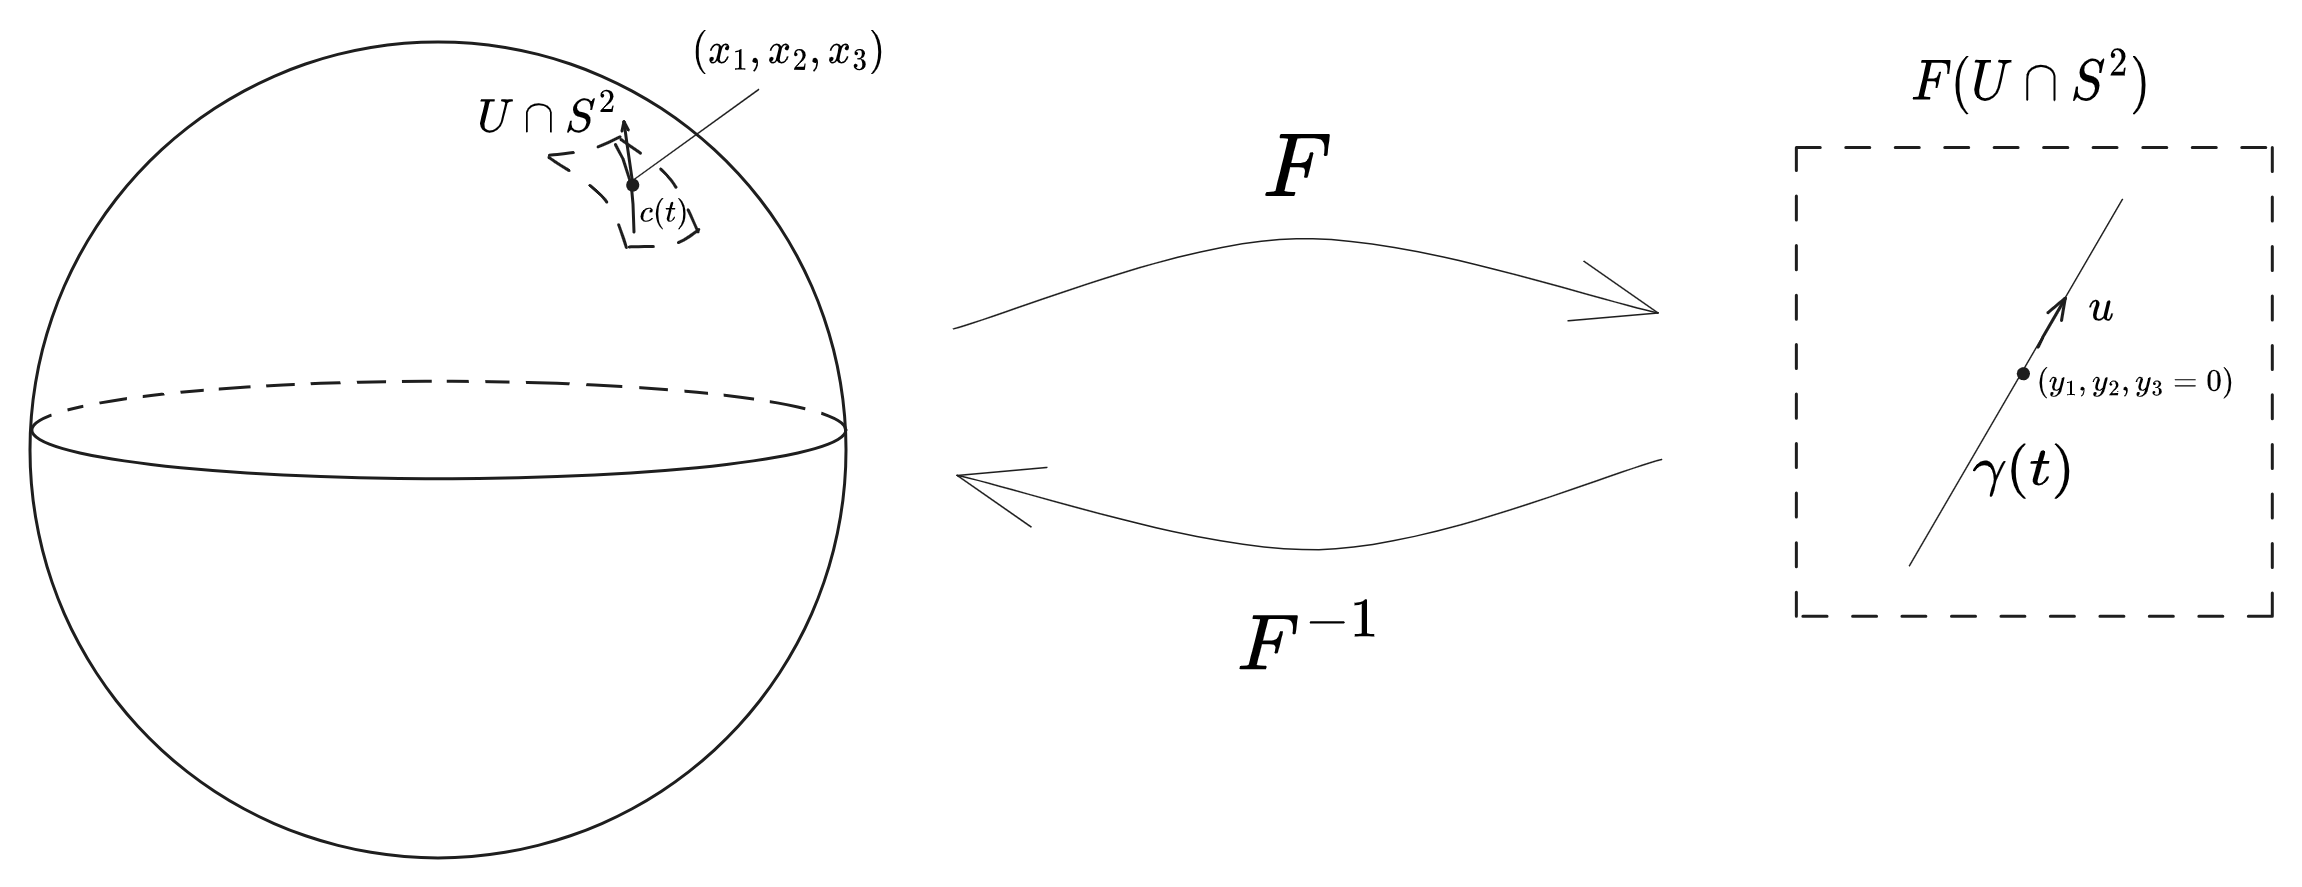
\includegraphics[width=0.7\textwidth]{figures/3.png}
    \centering 
\end{figure}
Consider $x = (x_1, x_2, x_3)$ and around that point, meaning in some neighborhood $U$ we have a diffeomorphism $F$ s.t. 
\begin{equation}
    F(U \cap S^2) = V \cap E 
\end{equation}
where $E = \{y \in \mathbb{R}^3 \ | \ y_3 = 0\}$ and $V$ is some neighborhood of $F(x)$. So it locally flattens the sphere. But this can also be interpreted as a change of coordinates 
\begin{equation}
    (x_1, x_2, x_3) \to F(x) = (y_1, y_2, y_3)
\end{equation}
In these new coordinates we can easily define straight path, which I denoted as $\gamma(t)$ with a given velocity vector $u$. In fact, it's a $3$-dimensional vector, but its third component is zero. Then we return back to the original coordinates and get the path $c(t)$ on a sphere. Of course the velocity vector will transform somehow, but this is not important as long as all such vectors form a vector space (in this case $2$-dimensional). In the proof of \textbf{Theorem 3.15} we will make this statement more formal, so let's finally get to the proof, which should now be fairly easy to understand. 

\begin{proof}[Proof of theorem 3.15]
$ $ 

\noindent \textbf{Part 1} For open submanifolds the central idea, is that with each $x \in \mathcal{M}$ there is an open ball $B(x; \varepsilon) \subseteq \mathcal{M}$, so for every $0 \neq v \in \mathcal{E}$ we can always take $I = \left(-\frac{\varepsilon}{\norm{v}}, \frac{\varepsilon}{\norm{v}}\right)$ and 
\begin{equation}
    c : I \to \mathcal{M}, \quad c(t) = x + tv 
\end{equation}
then $c(0) = x$ and $c^\prime(0) = v$. Thus, $\mathcal{E} \subseteq \T_x \mathcal{M}$ and so $\T_x \mathcal{M} = \mathcal{E}$. For $v = 0$ we can just take the "path" remaining at the same point $x$ for all $t \in I$. 

\noindent \textbf{Part 2} Consider the case of $\mathcal{M}$ an embedded submanifold of dimension $n = d - k$ with $k \geq 1$. Let $h: U \to \mathbb{R}^k$ be a local defining function of $\mathcal{M}$ around $x$. We will prove the result in two steps. 

The first step is straightforward, using the chain rule, we show that every $\T_x \mathcal{M} \subseteq \ker \D h(x)$. 

If $v \in \mathcal{M}$, then there exists $c : I \to \mathcal{M}$, smooth, s.t. $c(0) = x$ and $c^\prime(0) = v$. Since $c(t)$ is in $\mathcal{M}$ we have 
\begin{equation}
    h(c(t)) = 0
\end{equation}
both function are smooth, so we can apply the chain rule 
\begin{equation}
    \D h(c(t))[c^\prime (t)] = 0
\end{equation}
thus at $t = 0$ 
\begin{equation}
    \D h(x)[v] = 0
\end{equation}
and $v \in \ker \D h(x)$.

For the second step, using \textbf{Theorem 3.12} we will perform the coordinate transformation, construct the neccessary path for each $u \in \mathbb{R}^{d-k}$ similar to how we did it with $S^{1}$, which in turn implies that $\T_x \mathcal{M}$ contains a linear subspace of the same dimension as $\ker \D h(x)$. Then immediately $T_x \mathcal{M} = \ker \D h(x)$. 

\textit{Q: Is this obvious to everyone here? (if not, just refer to the basis vectors and step 1)}

We get diffeomorphism $F: U \to V$ from \textbf{Theorem 3.12} s.t. $U$ is a neighborhood of $x$ and 
\begin{equation}
    F(\mathcal{M} \cap U) = E \cap V 
\end{equation}
where $E = \{y \in \mathbb{R}^d \ | \ y_{n+1} = 0, ..., y_{d} = 0\}$, so $\dim E = \dim M$. For $u \in \mathbb{R}^{d-k}$ Define 
\begin{equation}
    \gamma: I \to \mathbb{R}^{d}, \quad \gamma(t) = F(x) + t \begin{bmatrix}
        u \\
        0_k 
    \end{bmatrix} 
\end{equation}
where $0_k$ is a zero vector of dimension $k$, and $I$ is picked so $\gamma$ remains in $E \cap V$ (open set). 

Now, let's define 
\begin{equation}
    c(t) = F^{-1}(\gamma(t))
\end{equation}
then $c(t) \in \mathcal{M}$ from $F^{-1}(E \cap V) = \mathcal{M} \cap U$ and our choice of $I$. Notice that 
\begin{equation}
    c(0) = F^{-1}(\gamma(0)) = F^{-1}(F(x)) = x
\end{equation}

Moreover, $F$ is a diffeomorphism, so $F^{-1}$ is smooth, and we can apply the chain rule again 
\begin{equation}
    c^\prime (t) = \D F^{-1}(\gamma(t))[\gamma^\prime (t)]
\end{equation}
in particular for $t = 0$ 
\begin{equation}
    c^\prime (0) =  [\D F^{-1}(F(x))] \begin{bmatrix}
        u \\
        0_k 
    \end{bmatrix} 
\end{equation}
and $[\D F^{-1}(F(x))] = (\D F(x))^{-1}$ is invertible from the inverse function theorem (which was used to prove \textbf{Theorem 3.12}). What's crucial, is that it only depends on $x$ and linear, so it's an isomorphism between $\mathbb{R}^{n}$ (where $u$ lives) and some subset of $\T_x \mathcal{M}$. This is exactly what we wanted to achieve step 2, and ends the proof. 

\end{proof}

Now we are confident in saying that 
\begin{definition}
    the previously defined $\T_x \mathcal{M}$ we call the tangent space to $\mathcal{M}$ at $x$. Vectors in $\T_x \mathcal{M}$ are called \textbf{tangent vectors}.
\end{definition}
In addition, it follows from the proof of the theorem 
\begin{equation}
    \dim \T_x \mathcal{M} = \dim \mathcal{M}
\end{equation} 
so the dimension of the tangent space is independent of $x$.

\setcounter{example}{16}

\begin{example}
    The linear space $\mathcal{M} = \mathbb{R}^{d}$ is a linear manifold of dimension $d$, because it's open in $\mathbb{R}^{d}$. It's tangent spaces $\T_x \mathcal{M} = \mathbb{R}^{d}$ are given by \textbf{Theorem 3.15 (1)}. 

    The affine space $\mathcal{A} = \{x \in \mathbb{R}^{d} \ | \ Ax = b\}$ defined by a matrix $A \in \mathbb{R}^{k \times d}$ or rank $k$ and arbitrary vector $b \in \mathbb{R}^{k}$ is a manifold of dimension $n = d - k$ embedded in $\mathbb{R}^{d}$. 
    \begin{proof}
        Define $h : \mathbb{R}^{d} \to \mathbb{R}^{k}$ as 
        \begin{equation}
            h(x) = Ax - b 
        \end{equation}  
        then $x \in \mathcal{A} \Leftrightarrow h(x) = 0$, and 
        \begin{equation}
            \D h[x] = A 
        \end{equation}
        so $\rank \D h(x) = \rank A = k$, which means that $h$ is a defining function for $\mathcal{A}$ for all $x$, and by definition $\mathcal{A}$ is a manifold. As for it's tangent space, we have by \textbf{Theorem 3.15 (2)}
        \begin{equation}
            \T_x \mathcal{A} = \ker \D h(x) = \ker A = \{x \in \mathbb{R}^{d} \ | \ Ax = 0 \}
        \end{equation}
    \end{proof}
\end{example}

\begin{example}
    The sphere $S^{d-1} = \{x \in \mathbb{R}^{d} \ | \ x^T x = 1\}$ is the zero level set of
    \begin{equation}
        h: \mathbb{R}^{d} \to \mathbb{R}, \quad h(x) = x^T x - 1 
    \end{equation}
    which is smooth. As we discussed 
    \begin{equation}
        \D h(x)[v] = 2x^T v 
    \end{equation}
    and for all $x \in S^{d}$ at least one coordinate is non-zero, so 
    \begin{equation}
        \rank \D h(x) = 1
    \end{equation}
    as a result $S^{d-1}$ is an embedded submanifold of $\mathbb{R}^{d}$ of dimension $n = d -1$. While it's tangent space is (again, by \textbf{Theorem 3.15 (2)})
    \begin{equation}
        \T_x S^{d-1} = \ker \D h(x) = \{v \in \mathbb{R}^{d} \ | \ x^T v = 0\}
    \end{equation}
\end{example}

\begin{example}
    Consider
    \begin{equation}
        \text{Sym}(2)_1 = \left\{X = \begin{bmatrix} x_1 & x_2 \\
        x_2 & x_3 \end{bmatrix} \ \Big| \ \rank X = 1\right\} 
    \end{equation}
    this is a subset of $\text{Sym}(2)$, the linear space of symmetric matrices of size two, that's diffeomorphic to $\mathbb{R}^3$. $\rank$ is not a smooth function, so it can't serve as a local defining function. However, it's possible to construct local defining function as follows. Let $U = \text{Sym}(2) \setminus \{0\}$, which is the open subset of $\text{Sym}(2)$. And consider 
    \begin{equation}
        h :  U \to \mathbb{R}, \quad h(X) = x_1 x_3 - x_2^2
    \end{equation}
    clearly $h$ is smooth, and $h^{-1}(0) = \text{Sym(2)}_1$. Furthermore
    \begin{equation}
        \D h(X)[\dot{X}] = x_3 \dot{x}_1 + x_1 \dot{x}_3 - 2x_2 \dot{x}_2 = \begin{bmatrix}
            x_3 & -2x_2 & x_1 
        \end{bmatrix} \begin{bmatrix}
            \dot{x}_1 \\
            \dot{x}_2 \\
            \dot{x}_3
        \end{bmatrix}
    \end{equation} 
    where $\dot{X}$ is a matrix in $\text{Sym}(2)$. This linear map has rank one provided $X \neq 0$, which is always the case in $U$. 
    Thus, $h$ is a defining function for $\text{Sym}(2)_1$ everywhere. Which confirms that $\text{Sym}(2)_1$ is a $2$-dimensional submanifold of $\text{Sym}(2)$. 
    
    \textit{Q: What's the geometric representation of this manifold?}

    \begin{equation}
        x_1x_3 - x_2^2 = \frac{1}{2} \left((x_1 + x_3)^2 - (x_1 - x_3)^2\right) - x_2^2 
    \end{equation}
    thus 
    \begin{equation*}
        x_1x_3 - x_2^2 = 0 \Leftrightarrow (x_1 + x_3)^2 = (2x_2)^2 + (x_1 - x_3)^2 
    \end{equation*}
    after the change of variables 
    \begin{equation}
        \begin{cases}
            z_1 = x_1 - x_3 \\
            z_2 = 2x_2 \\
            z_3 = x_1 + x_3 
        \end{cases}
    \end{equation}
    we get 
    \begin{equation}
        z_1^2 + z_2^2 = z_3^2 
    \end{equation}
    so it's an elliptic cone, but with excluded origin. It's not connected, neither open, nor closed. So it's a very non-trivial manifold in this sense. 
    
    However, we have enough machinery to study it. For example, it's tangent space at $X$ can be computed by \textbf{Theorem 3.15}. 
    \begin{equation}
        \T_X \text{Sym}(2)_1 = \{\dot{X} \ | \ x_3 \dot{x}_1 + x_1 \dot{x}_3 - 2x_2 \dot{x}_2 = 0 \}
    \end{equation}
\end{example}

\end{document}